\documentclass{beamer}
\usetheme{Berlin}
\usepackage{graphicx}

\title{Presentation}
\author{Tom Marx}

\definecolor{chocolate}{RGB}{33,33,33}

%\setbeamercolor{alerted text}{fg=orange}
%\setbeamercolor{background canvas}{bg=white}
%\setbeamercolor{block body alerted}{bg=normal text.bg!90!black}
%\setbeamercolor{block body}{bg=normal text.bg!90!black}
%\setbeamercolor{block body example}{bg=normal text.bg!90!black}
%\setbeamercolor{block title alerted}{use={normal text,alerted text},fg=alerted text.fg!75!normal text.fg,bg=normal text.bg!75!black}
%\setbeamercolor{block title}{bg=blue}
%\setbeamercolor{block title example}{use={normal text,example text},fg=example text.fg!75!normal text.fg,bg=normal text.bg!75!black}
%\setbeamercolor{fine separation line}{}
%\setbeamercolor{frametitle}{fg=brown}
%\setbeamercolor{item projected}{fg=black}
%\setbeamercolor{normal text}{bg=black,fg=yellow}
%\setbeamercolor{palette sidebar primary}{use=normal text,fg=normal text.fg}
%\setbeamercolor{palette sidebar quaternary}{use=structure,fg=structure.fg}
%\setbeamercolor{palette sidebar secondary}{use=structure,fg=structure.fg}
%\setbeamercolor{palette sidebar tertiary}{use=normal text,fg=normal text.fg}
%\setbeamercolor{section in sidebar}{fg=brown}
%\setbeamercolor{section in sidebar shaded}{fg=grey}
%\setbeamercolor{separation line}{}
%\setbeamercolor{sidebar}{bg=red}
%\setbeamercolor{sidebar}{parent=palette primary}
%\setbeamercolor{structure}{bg=black, fg=green}
%\setbeamercolor{subsection in sidebar}{fg=brown}
%\setbeamercolor{subsection in sidebar shaded}{fg=grey}
%\setbeamercolor{title}{fg=brown}
%\setbeamercolor{titlelike}{fg=brown}

\beamertemplatenavigationsymbolsempty

\begin{document}
\maketitle

\section{Introduction}

\begin{frame}
\frametitle{This is the first}
  \begin{itemize}
    \item Frames\pause
    \item Pauses and slides\pause
    \item Sections\pause
    \item Images
    \item Columns\pause
  \end{itemize}
\end{frame}

\section{Data}

\begin{frame}
  \frametitle{Images in Beamer}
  \framesubtitle{A bit more information about this}
  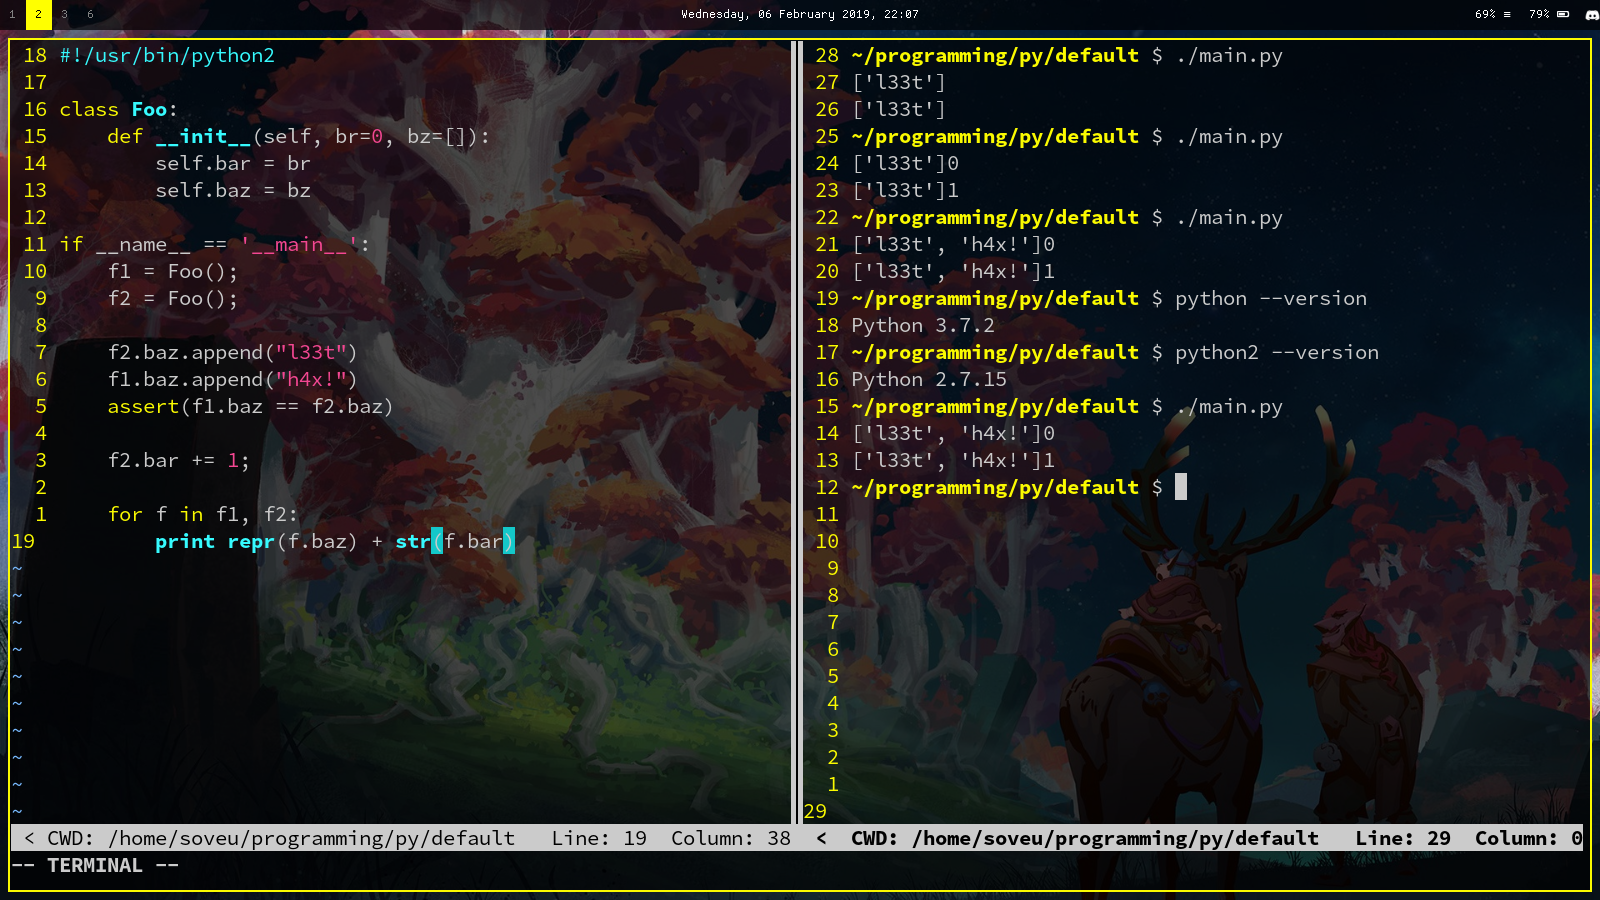
\includegraphics[width=\textwidth]{pybug23.png}
\end{frame}

\begin{frame}
\frametitle{Columns}
  \begin{columns}
    \column{.5\textwidth}
oiasjdoisadoiunhoidf jwqoid wqoiuias jdoiqwjdoijw qoidjwqoid jqoiwjdoqiw oiqwdjqwdqwdqwd
    \column{.5\textwidth}
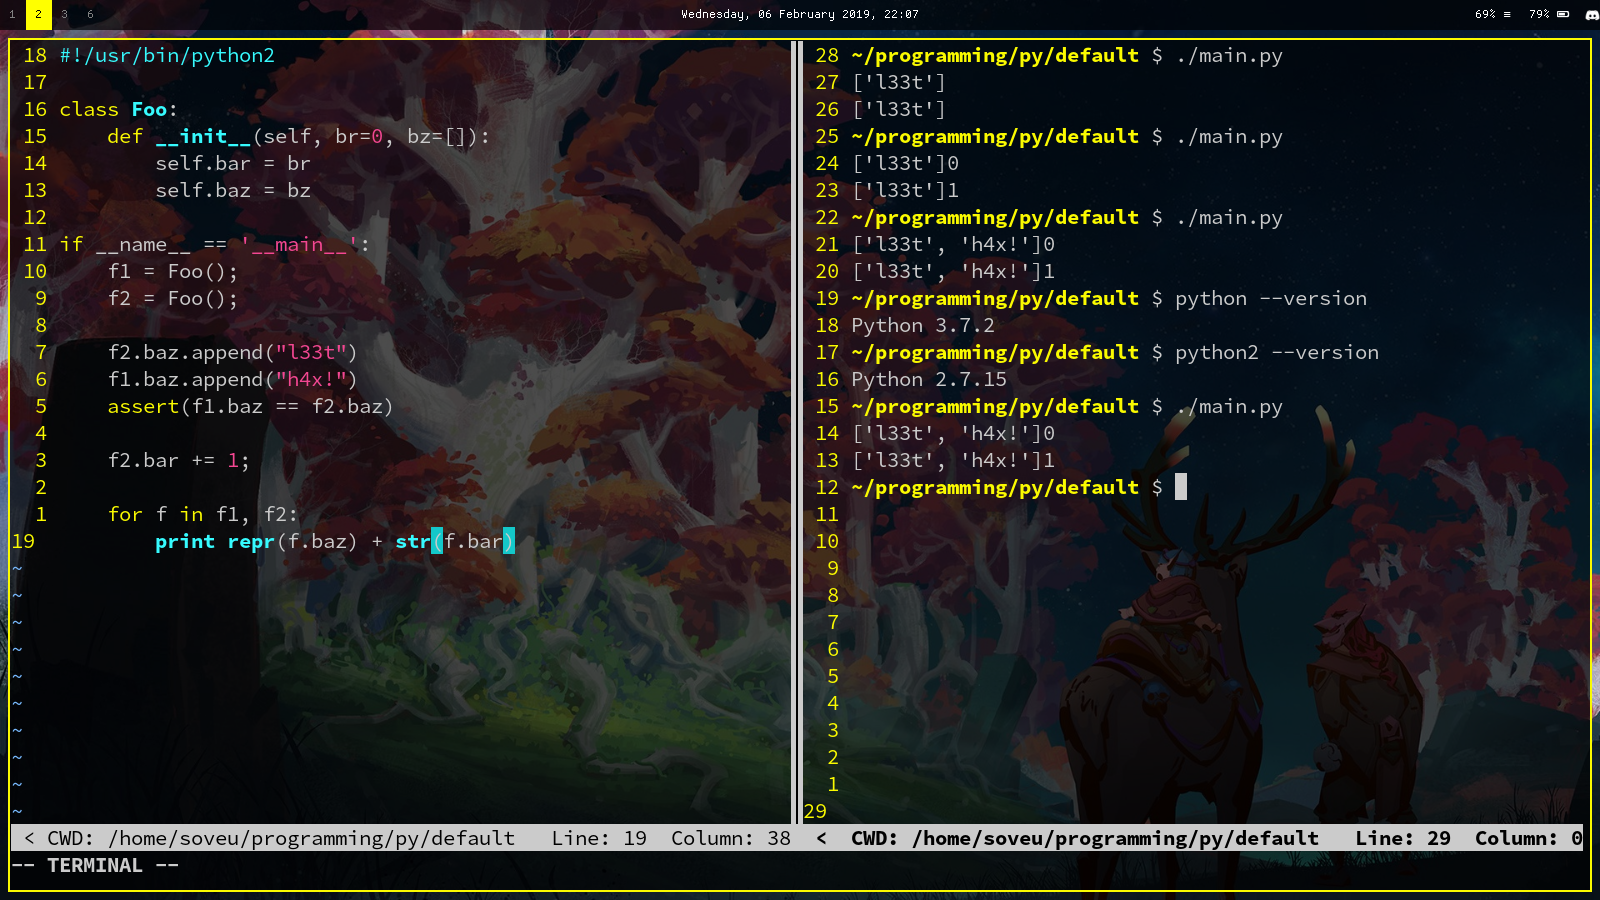
\includegraphics[width=\textwidth]{pybug23.png}
oiore igoirenjgio reefrefninpoasn joifnmjoivneoiu j32198rj3298r2 hjr928hr98
  \end{columns}
\end{frame}
\end{document}

